% begin-region: Preamble

%% Preamble is the part before \begin{document}.

%% Document type
\documentclass[12pt, a4paper]{article}

%% Packages
\usepackage{fontspec} % for custom fonts
\usepackage{geometry} % for page setup
\usepackage{graphicx} % for images
\usepackage{hyperref} % for URLs

%% Configuration
\geometry{margin=1in} % Set page margin

%% Metadata
\title{Learn \LaTeX{}}
\author{Prasanna, Venkatesh
	\thanks{
		\url{https://www.overleaf.com/learn/latex/Learn_LaTeX_in_30_minutes}
	}
}
\date{\today}

% end-region: Preamble

\begin{document}

\maketitle 

Hello there! I am learning \LaTeX.

% This is a comment

\tableofcontents

\section{Text formatting}

	\textbf{Bold}, \textit{italics}, \underline{underlined}. \textbf{\textit{\underline{Hey, I am all!}}}
	
	\subsection{\texttt{\textbackslash emph\{\}} command}
	
		\texttt{\textbackslash emph\{\}} applies correct emphasis based on the context.
		
		\bigskip
		
		\textbf{LaTeX:} \verb|This is \emph{my} book. \textit{No! This is \emph{mine}.}|
		
		\textbf{Output:} This is \emph{my} book. \textit{No! This is \emph{mine}.}
		
	\subsection{Small Caps}
	
		\textsc{This is in Small Caps.}
		
	\subsection{Verbatim}
	
		\verb|This is shown just as it is written i.e. \textit{verbatim}|. It is used for displaying code. For multiple lines, the \verb|verbatim| environment is used:
		
		\begin{verbatim}
			This is like HTML <pre> tag.
			\textbf{Bold}, \textit{italics}, \underline{underlined}. 
			\textbf{\textit{\underline{Hey, I am all!}}}
		\end{verbatim}


		The delimiter for \verb|\verb| can be any character other than * (astrieks)\footnote{\url{https://tex.stackexchange.com/a/203588}}\footnote{\url{https://webhome.phy.duke.edu/~rgb/General/latex/ltx-342.html}}.

\section{Font}

	\subsection{Serif}
	
		\textsf{I am without serif.} \textrm{I am with serif.}
		
	\subsection{Monospace}
	
		\texttt{I am teletype (tt) AKA monospace or typewriter.)} \textnormal{But I am normal AKA proportional.}

%	\subsection{Built-in Fonts}
%	
%		{\fontfamily{qcr}\selectfont This is a built-in sans-serif font.}
		
\section{Spacing}

	\subsection{Indent}
	
		First paragraph
		
		\noindent Second paragraph
		
\section{Images}

	\verb|\includegraphics{}| command from \verb|graphicx| package is used to add images.
	
	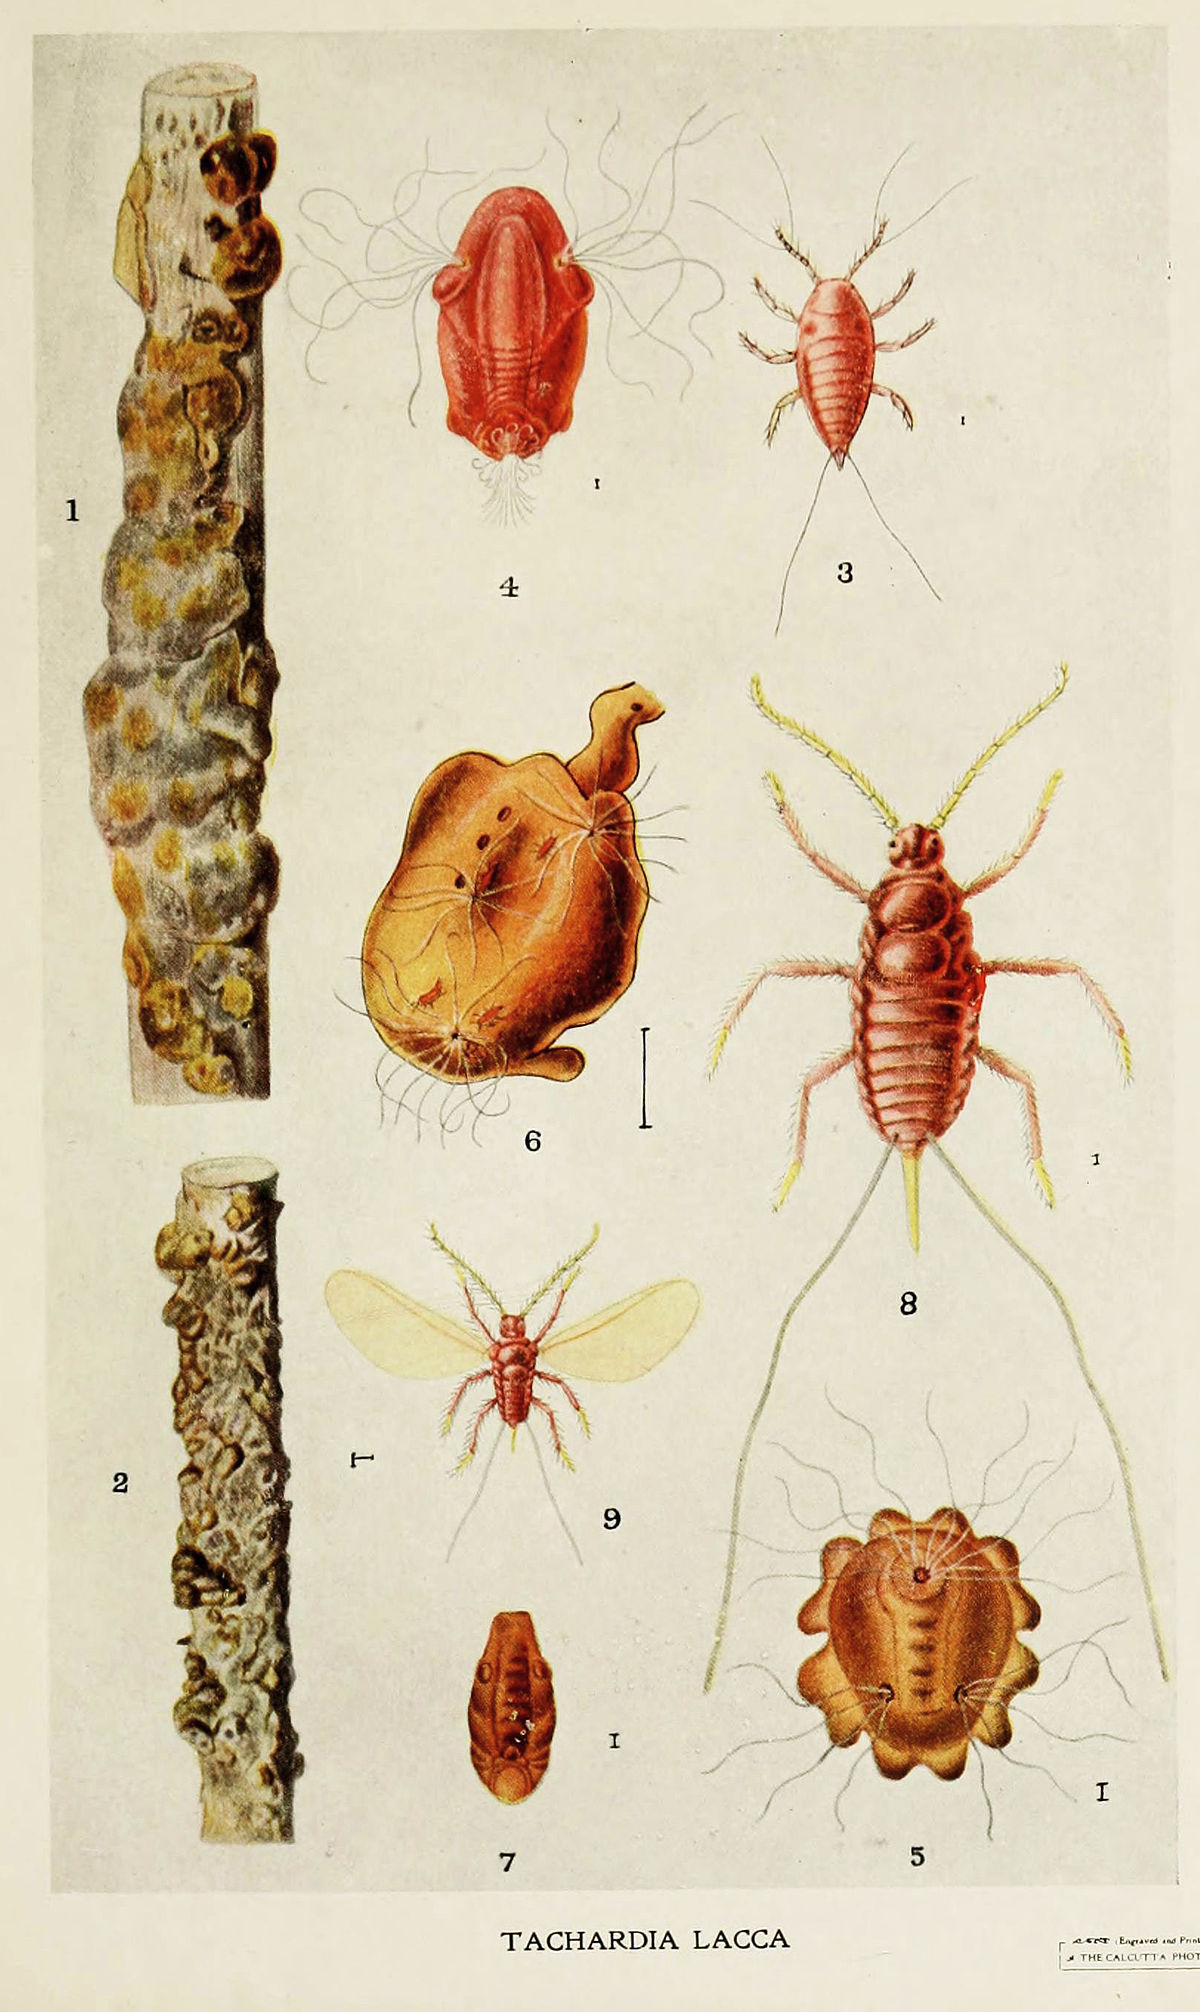
\includegraphics[height=5cm]{./images/Kerria-Lacca}
	
	\subsection{Image with Caption and Reference}
	
		The \verb|figure| environment is used to captions, labels, and references. See Figure \ref{fig1}.
	
		\begin{figure}[h]
			\centering
			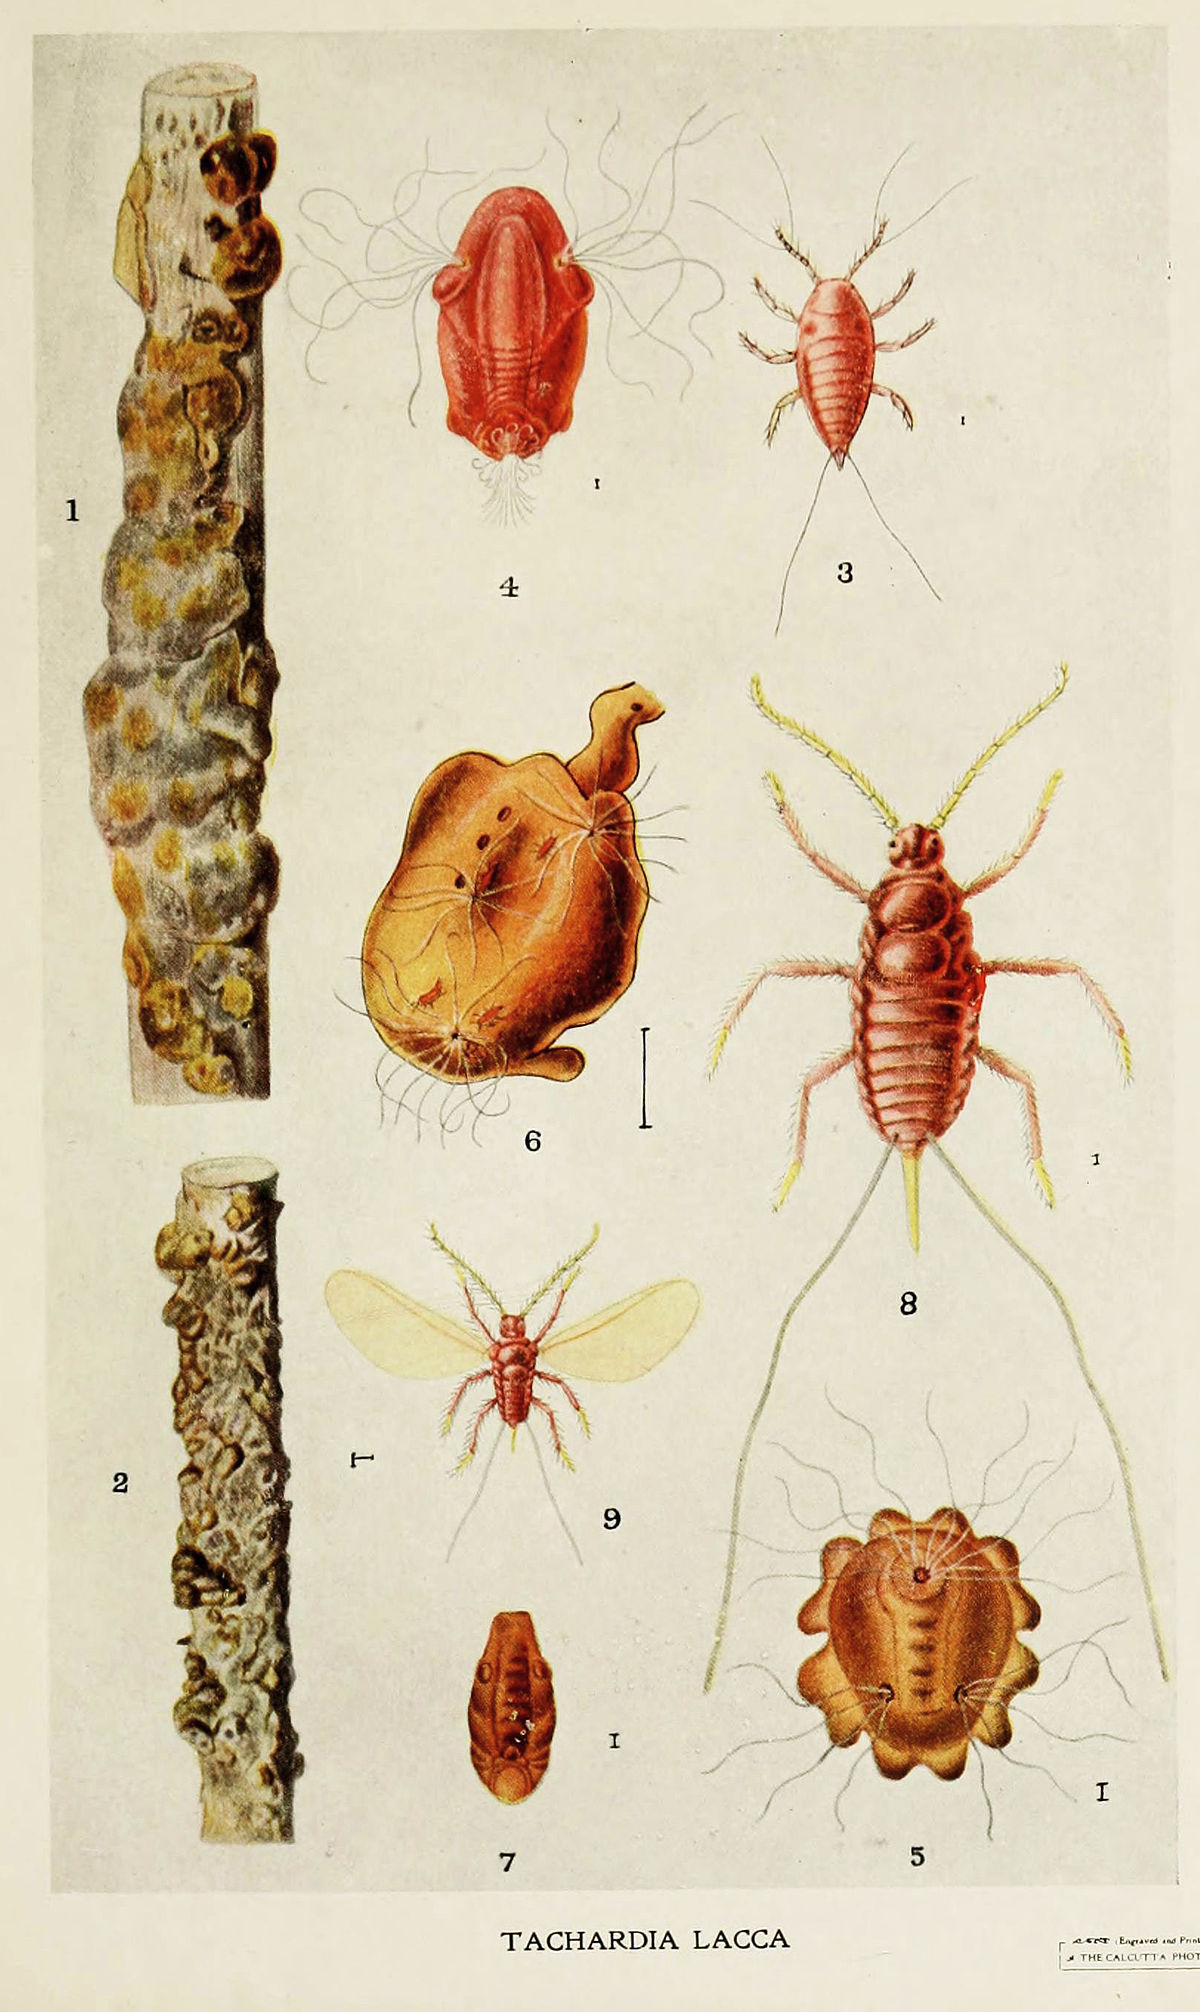
\includegraphics[height=5cm]{./images/Kerria-Lacca}
			\caption{This image is in figure environment and has caption.}
			\label{fig1}
		\end{figure}

\section{Enviroment}

	Environments are sections of our document that you want to present in a different way to the rest of the document.\footnote{\url{https://www.overleaf.com/learn/latex/Learn_LaTeX_in_30_minutes\#Creating_lists_in_LaTeX}}
	
	\begin{verbatim}
		\begin{environment-name}
			content
		\end{environment-name}
	\end{verbatim}
	
	\subsection{List}
	
		\subsubsection*{Unordered List}
		
		\begin{itemize}
			\item Item one
			\item Item two
			\item Item three
			\item Item four
		\end{itemize}
	
		\subsubsection*{Ordered List}
		
		\begin{enumerate}
			\item First item
			\item Second item
			\item Third item
			\item Fourth item
		\end{enumerate}
	
\section{Sections}

	This is a section.

	\subsection{Subsection}
	
		This is a subsection.
	
	\subsubsection{Subsubsection}
	
		This is a subsubsection.
	
	\subsection*{Unnumbered Section}
	
		\verb|\section*{text}| (Section command with *) is used to create unnumbered section. Similarly, for subsection and subsubsection.
	
	\subsection*{Unnumbered Section with TOC entry}
	\label{sec:unnumbered}
	\addcontentsline{toc}{subsection}{\nameref{sec:unnumbered}}
	
		Unnumbered *sections are not added to the TOC. An unnumbered *section can be explicity added to the TOC using \verb|\addcontentsline| command. See section, "\nameref{sec:unnumbered}".
	
\section{Tables}

	\subsection{Simple Table}
	
		\begin{tabular}{c c c}
			cell 1 & cell 2 & cell 3 \\
			cell 4 & cell 5 & cell 6 \\
			cell 7 & cell 8
		\end{tabular}
	
	\subsection{Right and Left-aligned Columns}
	
		\begin{tabular}{l c r}
			right-aligned 	& center-aligned 	& left-aligned \\
			cell 4 			& cell 5 			& cell 6 	   \\
			cell 7 			& cell 8
		\end{tabular}
	
	\subsection{Center-aligned Table}
	
		\begin{center}
			\begin{tabular}{l c r}
				right-aligned 	& center-aligned 	& left-aligned \\
				cell 4 			& cell 5 			& cell 6 	   \\
				cell 7 			& cell 8
			\end{tabular}
		\end{center}
	
	\subsection{Table with Borders}
	
		\subsubsection*{Vertical Borders}
		
			\begin{center}
				\begin{tabular}{|l|c|r|}
					right-aligned 	& center-aligned 	& left-aligned \\
					cell 4 			& cell 5 			& cell 6 	   \\
					cell 7 			& cell 8 			&\\
				\end{tabular}
			\end{center}
		
		\subsubsection*{Horizontal Borders}
		
			\begin{center}
				\begin{tabular}{l c r}
					\hline
					right-aligned 	& center-aligned 	& left-aligned \\
					\hline
					cell 4 			& cell 5 			& cell 6 	   \\
					cell 7 			& cell 8 			&\\
					\hline
				\end{tabular}
			\end{center}
		
		\subsubsection*{Both Borders}
		
			\begin{center}
				\begin{tabular}{|l|c|r|}
					\hline
					right-aligned 	& center-aligned 	& left-aligned \\
					\hline
					cell 4 			& cell 5 			& cell 6 	   \\
					\hline
					cell 7 			& cell 8 			&\\
					\hline
				\end{tabular}
			\end{center}
		

	\subsection{Table with Caption and Reference}
	
		The \verb|table| environment is used to add captions, labels and references. See Table \ref{tab1}.
		
		\begin{table}[h]
			\centering
			\begin{tabular}{|l|c|r|}
				\hline
				right-aligned 	& center-aligned 	& left-aligned \\
				\hline
				cell 4 			& cell 5 			& cell 6 	   \\
				cell 7 			& cell 8 			&\\
				\hline
			\end{tabular}
			\caption{This table is in \texttt{table} environment and has a caption.}
			\label{tab1}
		\end{table}

\end{document}